\documentclass{article}[11pt,subeqn]

\title{The Twin Instrument\footnote{We are grateful to Paul Devereux, James Fenske, 
Atheen Venkataramani and Cheti Nicoletti,  [WHO ELSE TO ADD?] along with seminar 
audiences and discussants at CMPO Bristol, 
ESPE, NEUDC, CSAE, and The University of Essex for helpful comments.  We make full data and
source code available for examination and replication.  This is available at
\texttt{https://bitbucket.org/damiancclarke/twins}.}}
\author{Sonia Bhalotra\thanks{The University of Essex.  Contact: srbhal@essex.ac.uk} 
\and Damian Clarke\thanks{The University of Oxford.  Contact: damian.clarke@economics.ox.ac.uk}}
\date{\today}

\usepackage[capposition=top]{floatrow}
\usepackage{url}
\usepackage{longtable}
\usepackage{booktabs}
\usepackage{rotating}
\usepackage{dcolumn}
\usepackage{color}
\pagecolor{white}
\usepackage{pdfpages}
\usepackage{lastpage}
\usepackage{lscape}
\usepackage{setspace}
\usepackage{amsmath}
\usepackage{amssymb}
\usepackage{breqn}
\usepackage{appendix}
\usepackage{natbib}
\bibliographystyle{abbrvnat}
\bibpunct{(}{)}{;}{a}{,}{,}

\usepackage{caption}
\usepackage{subcaption}

\usepackage{epsfig}
\usepackage{epstopdf}
\usepackage{multirow}

\usepackage{wrapfig}
\usepackage{blindtext}

\setlength\topmargin{-0.375in}
\setlength\textheight{8.8in}
\setlength\textwidth{5.8in}
\setlength\oddsidemargin{0.4in}
\setlength\evensidemargin{-0.5in}
\setlength\parindent{0.25in}
\setlength\parskip{0.25in}

\newcommand{\person}{we\ }
\newcommand{\Person}{We\ }

\bibliographystyle{abbrvnat}
\bibpunct{(}{)}{;}{a}{,}{,}

\newcommand\independent{\protect\mathpalette{\protect\independenT}{\perp}}
\def\independenT#1#2{\mathrel{\rlap{$#1#2$}\mkern2mu{#1#2}}}

\usepackage{changepage}% http://ctan.org/pkg/changepage
\makeatletter
\newenvironment{chapabstract}{%
    \begin{center}%
      \bfseries Abstract
    \end{center}}%
   {\par}
\makeatother


\newcommand{\twinfolder}{./../../../Twins}
\newcommand{\biblioinc}{\newpage \bibliography{./../../Document/ThesisRefs}}

\begin{document}
\begin{spacing}{1.4}

\maketitle
\begin{abstract}
 The incidence of twins has been used to identify the impact of changes in fertility 
 on measures of investment in children born prior to the twins, and the emerging 
 consensus in this literature is that there is no evidence of a quantity-quality 
 trade-off. We argue that the standard approach is flawed for two reasons. First, 
 even if twin conception is random, bringing twins to term is a function of maternal 
 health which is difficult to fully observe and which tends to be correlated with 
 child quality, rendering the instrument invalid. Second, twins will only constitute 
 a shock to family size if their occurrence takes family size across the desired 
 level. The neglect of both of these considerations in the literature will tend to 
 lead to under-estimation of the quality-quantity (Q-Q) trade-off and so could 
 contribute to explaining the negative results in the literature. Using a large sample
 of microdata from developing countries, we show that a significant trade-off emerges
 upon correcting for these biases.  We show that this result is likely to be only a 
 \emph{lower} bound of the true Q-Q trade-off and discuss how to estimate the size of
 these bounds. \\
\end{abstract}

\hspace{4mm}\textbf{\small JEL codes}: J13,J16,J18,I15,O15. \\
\newpage
\section{Introduction}
%********************************************************************************
Since the pioneering work of \citet{RosenzweigWolpin1980}, economists have 
attempted to leverage the occurrence of twin births to estimate the effect of 
family size on child outcomes. If twin births occur at random, the occurrence of 
twin births constitutes a fertility shock that is uncorrelated with family 
characteristics including parental preferences, and other unobservables which may 
be related to child quality. This provides the exogenous variation (in quantity) 
required to estimate the quantity-quality model of \citet{Becker1960,
BeckerLewis1973,BeckerTomes1976}.  The essential idea is that the shadow price of 
child quality is increasing in child quality and \emph{vice versa} i.e.\ the 
shadow price of quantity is increasing in quality.  By comparing those families who 
unexpectedly produced additional children to those who always produced one child
per birth, we can isolate the effect of an individual's sibling size on her human 
capital attainment.

However, the consistent estimation of this effct is based upon the untestable 
assumption that twinning is exogenous. This requires not only that twin conceptions 
are randomly assigned to families, but also that taking a twin conception to term 
does not depend upon a woman's behaviours during pregnancy or on her endowments
prior to pregnancy. This is at odds with the evidence.

We show that endowments and behaviours affect the chances of twins being born (see 
section \ref{TWINscn:results} below and \citet{BhalotraClarke2014}). In data from 
a large sample of developing countries, we show that taller women and women with a 
higher body-mass index are significantly more likely to give birth to twins.\footnote{
Height is an index of the stock of health of a woman and is a function of investments 
over her growth period and, especially, the early years of her life (see references 
in \citet{BhalotraRawlings2013})} Maternal health is likely to be an especially significant 
determinant of birth outcomes in poorer countries where many women are chronically 
under-nourished (an indicator of which is their final stature), exhibit anemia and 
low-BMI and are prone to infections. In these conditions only relatively healthy 
women will have the resources to support a successful twin pregnancy. However, our 
critique applies to richer countries too. Using data from the UK, Scotland, the USA 
and Chile, we find that women who are taller and less likely to engage in risky
behaviours such as smoking, drug taking or alchol consumption during pregnancy are 
significantly more likely to have a (live) twin birth.\footnote{Simiarly, it is 
well known that fertility treatments increase the likelihood of twinning. While we 
do not discuss this extensively here, we note that this is likely to be less of an 
identification challenge given that IVF treatment is an entirely observable 
behaviour.}

Overall, our argument is that women who give birth to twins are positively selected and 
that the common tendency to ignore this will result in under-estimation of the QQ 
trade-off. We focus upon maternal health because no previous work has highlighted it 
as a determinant of twinning and because it is inherently impossible to fully control 
for. Even if we had data that included all of the indicators of health we mention 
above, we may not observe whether women skip breakfast \citep{MazumderSeeskin2014}, 
whether they are stressed (\citet{Blacketal2014} and references therein), whether they 
seek and adhere to antenatal care and so on.  Our contention adds a novel twist to a 
recent literature which suggests that mothers' health and fetal environment matter and 
may alter the birth weight of children, the sex ratio at birth and a range of future 
human capital outcomes \citep{Almondetal2011,BhalotraRawlings2013,Barker1995}. Like 
birth weight and the probability of a boy relative to a girl birth, the probability 
of a twin birth is increasing in the health of the mother/ the fetal environment.  

The emerging consensus in the literature using twin births to test the Q-Q model is 
that there is in fact no significant or substantial trade-off between fertility and 
investments in children. In this paper we suggest that this result may, in principle, 
follow from the bias created by twin-mothers being positively selected. We re-examine 
the validity of these results, accounting for the innovation discussed previously.
If twin births are not truly exogenous, but instead depend upon maternal health stocks 
and behaviours, there is an identification challenge.  Specifically, if healthier 
mothers are both more likely to give birth to twins, and more likely to invest in child 
human capital in later life, existing estimates may significantly underestimate the
size of the Q-Q tradeoff.  When ignoring these considerations we find that the effect 
of an additional birth on human capital attainment (education) is minor, or even 
weakly positive. However, when taking into account this innovation we find that a 
significant trade-off does exist, and that an additional birth reduces standardised 
schooling behaviour by at least 4\% of a standard deviation.

the estimated effect of $\sim 4\%$ of an s.d.\ is at most the lower bound for the true 
size of the Q-Q tradeoff. Given that we suggest that maternal health predicts twinning,
and given that maternal health is multidimensional in nature and difficult to observe 
fully, we will only ever be able to include a partial set of controls to account for 
the inconsistency in IV estimates. As such, we examine a number of methods to estimate 
plausible bounds on the Q-Q tradeoff. First, we argue that the true estimate is 
bounded by the OLS and IV estimtes. We also follow \citet{Conleyetal2012} in
conceptualizing twins as a plausibly exogenous event, and derive estimates by assuming 
that the traditional exclusion restriction is `close to' holding.

This work which further probes the Q-Q tradeoff is important, especially in the 
developing country setting on which we focus. In order to conduct empirical tests, 
we construct a large microdata set from 68 developing countries with observations on 
more than 2.5 million children and nearly 1 million mothers. The macro level trends in 
this data suggest that educational attainment has risen considerably while completed 
and desired fertility has fallen sharply over the past 50 years (see figures 
\ref{TWINfig:fertrend} and \ref{TWINfig:eductrend}). Similar effects have been described 
extensively in the empirical literature (ie \citet{Hanushek1992}). It is of considerable 
relevance to researchers and to policy makers to determine whether such a trend is (at 
least partially) causal. A significant number of countries have engaged in aggresive 
fertility control policies over the previous century, with family planning still 
considered a concern according to policy makers in the developing world.\footnote{A 
recent survey of national governments suggests that fertility was perceived as too 
high in 50\% of developing countries, with this figure rising to 86\% among the least 
developed countries \citet{UN2010}.} As discussed, our evidence suggests that the same 
identification problem arises with using twins as an instrument for fertility in 
analysis of data from richer countries. Future work is merited that assesses the size 
of the bias.\footnote{The data for Israel and China analysed in the twin-IV studies of 
\citet{Angristetal2010} and \citet{RosenzweigZhang2009} respectively do not contain 
information on maternal health. The data for Norway analysed in the twin-IV study of 
\citet{Blacketal2005} are not accessible outside Norway.}

This paper unfolds as follows.  In the next section we discuss the existing 
literature which estimates the Q-Q model using twins.  We then discuss the large
dataset that we will use to examine twin exogeneity and to bound the Q-Q tradeoff.
Section \ref{TWINscn:method} discusses our methodology, while section 
\ref{TWINscn:results} presents results.  We briefly conclude in the final section.


\section{The Twin Literature}
%********************************************************************************
The occurrence of twin births is a commonly used for identification in economic
studies.  Typically, these assume that twinning is (at least conditionally) 
exogenous.


\section{Data}
The data used here come from the Demographic and Health Surveys (DHS).  The DHS 
are a set of nationally representative surveys which have been administered in 
low- and middle-income countries between 1985 and the present.  Women aged 
between 15--49 in surveyed households respond to an in-depth series of questions 
reporting their full fertility history (listing all surviving and non-surviving 
children), their actual and desired contraceptive use and number of births, 
education level, marital status, plus the measurement of a number of health 
endowments such as height and body mass index.  For all other members living in 
the household a shorter series of responses are recorded, including the 
individual's educational attainment.

This results in two distinct sets of data to be merged.  One database contains
one line for each birth reported by every 15--49 year-old woman surveyed with
a limited number of child-level covariates such as the child's date of birth,
type of birth (single or multiple), and the child's survival status.  The other
database contains one line for each member currently living in the survey 
household.  This database includes each member's educational status.  By 
crossing these two databases we are thus able to generate data for the
educational attainment of each of a woman's children currently residing in the 
household as well as their mother's health and educational status.  This 
database is selected in two ways: firstly it only contains children who have 
survived up until the survey date, and secondly it only contains children who 
have remained living in the same household as their mother.  In order to ensure 
that this sample is as representative as possible, we restrict our analysis to 
those children aged 18 and under.

We pool all publicly available DHS data resulting in microdata on 3,297,318
children ever-born to women who responded fully to any DHS survey.  A full list 
of the DHS countries and years of surveys which make up this sample is provided 
as appendix table \ref{TWINtab:countries}.  Of the 3,297,318 offspring reported in 
survey data, 2,033,510 remain living in the same household as their mother.  The 
majority of these 2,033,510 children are aged 18 and under (92.96\%) and hence make 
up our principal estimation sample (in future we will refer to this as the 
`household sample').  The remaining 1,263,808 offspring were not recorded as 
living in the same household as their mother.  Of these children \emph{not} in the 
household, and hence for whom education is not recorded, the majority (53.9\%) were 
aged over 18 or had died prior to the date of survey.\footnote{Children aged under 
18 who are alive but not living in the same household as their mother are 
statistically quite different to those children who do remain in the household.  
In our data sample, they are on average 2.7 years older, born to less educated 
and younger mothers, and are slightly more likely to be males or twins.}
%********************************************************************************



\section{Methodology}
Typically, empirical analyses of the quality-quantity trade-off focus on 
producing consistent estimates of $\beta_1$ in the following specification:
\begin{equation}
\label{TWINeqn:secondstage}
educ_{ij}=\beta_0+\beta_1 fert_{j} + \bm{X}\bm{\beta}_2+u_{ij}.
\end{equation}
Here, quality is proxied by the educational attainment of child $i$ in family 
$j$, ($educ$) and fertility ($fert$) is measured as the total births in a child's
family.  A vector of family and child controls is included, denoted $\bm{X}$.  As
has been extensively discussed in prior literature, estimation of $\beta_1$ using
OLS and cross-sectional data will result in biased coefficients given that child 
quality and quantity are jointly determined \citep{BeckerLewis1973,BeckerTomes1976}, 
and given that unobservable parental behaviours and attributes influence both 
fertility decisions, and investments in children's education \citep{Qian2009}.



\section{Results}
\subsection{Twin Exogeneity}
%*******************************************************************************
Table \ref{TWINtab:comp} presents a test of balance of maternal characteristics
between mothers who have and who have not given birth to twins.

In table \ref{TWINtab:twinreg1} we report the results from specification 
(\ref{TWINeqn:twinreg}). These results suggest that twin births are 
not random, even after conditioning on maternal age and child birth order as is
typical in recent twin literature. The inclusion of a full set of country and 
year-of-birth dummies (not displayed in table \ref{TWINtab:twinreg1}) will 
capture any systematic trend in the frequency of twin births across time or 
regions, and country dummies will absorb all time invariant differences in the 
probability of a twin birth across countries.  The estimated coefficients and 
signs support the idea discussed in section \ref{TWINscn:method} that higher 
`investments' (for example in maternal health) required to maintain multiple 
healthy fetuses \emph{in utero} may result in non-random twin births. Initially 
results from the pooled DHS data are presented as this provides a particularly 
large sample with which to test the hypothesis of twin exogeneity.  This is 
represented in table \ref{TWINtab:twinreg1} column (1) and provides considerable 
evidence that live multiple births respond to family `choice' variables such as 
education (tests for the joint significance of both socioeconomic variables and 
health variables are rejected with p-values of 0.0000).


The fact that maternal health is correlated with twinning is supported by medical 
literature, although is not a point that has been incorporated into prior 
economic studies of twinning.  \citet{Hall2003} for example suggests that 
follicle-stimulating hormone (FSH) is associated with an increased likelihood 
of twinning, and is found in higher concentrations in older, heavier and taller 
mothers.  Further, she suggests ``that adequate maternal folic acid consumption 
could affect the number of twins coming to term'' (see p.\ 741, and further 
discussion in \citet{Lietal2003}).  Given that twinning also increases in cases 
where the mother undergoes fertility treatment, we run a similar regression for 
children born in a period not potentially affected by IVF.\footnote{In order to 
be conservative, we estimate for the period preceeding 1990, the date which 
coincides with the first reported successful use of IVF in South Africa, an 
early-adopter among DHS countries.}  These results are included in columns (4) 
and (5), and although education is now no longer always significant, mother's 
height and weight, and family socioeconomic variables remain economically and 
statistically significant.

If the reason non-random twin births are observed is due to insufficient investment 
in the developing fetus, it seems likely that twin `selection' will be more 
pronounced in lower income settings, and settings where the mother is less well 
resourced during gestation.  This is tested in columns (2) and (3), where it is 
shown that the violation of the twin exclusion restriction is particularly strong 
in low income countries.  Here maternal health is a more important predictor, and 
the explained portion of this set of variables is larger that in middle-income 
countries.\footnote{The low $R^2$ in these regressions is not at all surprising 
given that twin conception can be thought of as an approximately random process.
The fact that socioeconomic and health variables have \emph{any} power in 
explaining twin birth however is sufficient to invalidate IV estimations if these 
or other relevant predictors are not controlled for.}

These results call into question the veracity of the conditional exogeneity (or 
`as good as random') assumption required to estimate $\beta$ consistently in 
(\ref{TWINeqn:secondstage}).  This implies that omitting factors such as family 
income...


\subsection{Twinning and Quantity-Quality}
%********************************************************************************
As is typically found in empirical studies of the Q-Q tradeoff, correlations 
between family size and child outcome variables are negative, and strongly 
significant. Table \ref{TWINtab:OLS} shows OLS estimates of child `quality' on
total fertility. These results suggest that an additional sibling is associated
with an approximatelty 0.1 sd decrease in standardised schooling outcomes.

Of course, this empirically observed relationship between the quantity of an 
individual's siblings and their measured `quality' does not necessarily imply 
that such a trade-off exists if parental decisions regarding the production of 
child quality and quantity are jointly made and possibly influenced by unobserved
factors \citep{BeckerTomes1976}.  Principally here we are concerned with 
unobserved parental behaviours which may favour both lower family size and higher 
child quality.  The OLS results are consistent with such a result, as the 
inclusion of maternal education and maternal health controls---likely correlated 
with desires for smaller family size and higher investments per child---reduce the 
magnitude of this observed trade-off.

%********************************************************************************
\subsubsection{Q-Q Tradeoff: Estimates Using Twin Births}
Rather than focusing on OLS estimates which are likely to be biased, we turn 
to estimates which rely on twin births to identify the Q-Q tradeoff.  As we 
outline in section \ref{TWINsscn:twinRes}, the assumption of `as good as random' 
twin births is unlikely to hold, even when conditioning on the augmented set of 
controls proposed in (\ref{TWINeqn:twinreg}).  If this is the case, we will 
also be unable to consistently estimate $\beta_1$ using twin births.

However, it is likely that the $\beta_1$ that we estimate using twin births will 
provide us with a strict lower bound of the magnitude of the Q-Q trade-off as
outlined in (\ref{TWINsscn:methodQQ}). We expect that the bias in this estimate 
is due to those mothers who invest more in their children in utero, or who have
greater initial health endowments, being more likely to give birth to twins 
resulting in larger family sizes.  At the same time, we expect healthier mothers 
to invest more in their children after birth resulting in higher quality children.
By relegating health variables to the error term, these two positive correlations 
will result in a positive bias on the fertility coefficient estimated via IV.  In 
order to determine the effect that these omitted variables have on estimates of 
the Q-Q trade-off, we turn to results for equation (\ref{TWINeqn:secondstage}), 
both first omitting, and the including, maternal health and socioeconomic 
variables.

We present IV estimates of the Q-Q trade-off in table \ref{TWINtab:IVAll}.  The 
main specification is displayed in the top row with separate columns for the 2+, 
3+ and 4+ sample groups.  In each case the base case (controlling for maternal 
and child age, country, and year of birth) results in insignificant, and at times 
weakly positive, estimates of the effect of an additional birth on a child's
educational attainment.  These results suggest that the inclusion of maternal 
health and socioeconomic controls may be of considerable importance.  Despite
the lack of results when using the `typical' set of twin controls, including 
health (columns 2, 4 and 6) reduces point estimates on fertility from an effect
of approximately 0\% of a standard deviation, to $-3$ or $-4$\% of a standard 
deviation in standardised educational attainment.  Further, conditioning on
maternal education results in slightly more precise estimates, suggesting a
statistically significant\footnote{Or close to statistically significant in the 
case of the 2+ sample.} Q-Q trade-off of at least 3 or 4\%.

%********************************************************************************
\subsubsection{Heterogeneity of the Q-Q Trade-off}
Estimates of the Q-Q trade-off are heterogeneous across birth orders, country 
income level, and gender of the child affected by the additional birth.  Such a 
result is not surprising if parents perceive that returns to education vary for 
different children or in different circumstances, and invest in human capital in 
line with this.  

The magnitude and significance of the results is lowest when considering the 
effect on the first-born child of moving from two to three births (the 2+ group), 
and higher when considering moving from three to four births or four to five 
births.  However, in lower fertility environments the effect is, as expected, 
concentrated on lower birth orders. The third row of table \ref{TWINtab:IVAll} 
suggests that in middle-income countries that the effect is largest on first 
borns, and progressively smaller, but still considerable, at higher birth orders.

Estimates of the magnitude of the Q-Q trade-off by country income level suggest
that the trade-off is considerably larger in \emph{middle} rather than low-income
countries.  In low-income countries point estimates on fertility suggest 
(insignificant) trade-offs centred around 2-3\% of a standard deviation, while 
in middle-income countries results are significant, and considerably larger,
reaching as much as 9\% of a standard deviation: only slightly lower than OLS
estimates for this group. [ADD TEST HERE LOOKING AT COSTS OF EDUCATION?  HIGHER
IN COUNTRIES WHERE EDUCATION COSTS MORE? SONIA, DO YOU HAVE THE EDUCATION COST 
DATABASE THAT I THINK YOU MENTIONED TO ME ONCE?]

Similarly, effects of the Q-Q trade-off are considerably different depending
upon a child's gender.  In table \ref{TWINtab:IVgend} we present specifications 
estimated separately by the gender of the index child.  These results suggest
that females may bear the brunt of additional births, with estimates being 
negative and significant for girls, while insignificant for boy children.  Such 
a result suggests that parents may engage in redistributory behaviour.  This 
idea has been extensively studied by \citet{RosenzweigZhang2009}, however their 
analysis focuses on the possibility that parents reinforce positive birth 
endowments based on child health, not based on child gender as we find here.

In order for the results we produce to be comparable to recent literature we
thus far have only focused on children \emph{preceding} twins.  As an 
alternative specification we also include the $n^{th}$ birth in the analysis
sample.\footnote{In the case of of the 2+ group we thus compare first and 
second born children from families which did not have a twin at the second
birth to first and second born children from families which did have a twin
at the second birth.}  Given the lower birth endowments of twins (and potential
that reinforcing behaviour moves resources away from twins as per 
\citet{RosenzweigZhang2009}), we expect to see that the trade-off is 
significantly stronger when including twins in the sample.  These results are 
displayed in the final row table \ref{TWINtab:IVAll}, and suggest that, if we 
focus not just on pre-twins, that the trade-off of an additional birth is large: 
on the order of 5-8\% of a standard deviation. Finally, in row 4 of the table
we perform an alternative consistency check.  Rather than using the full 
fertility reported by a family, we adjust birth order and fertility to only 
account for those children who survived beyond 1 year of age.  Once again, we 
find that the estimated Q-Q trade-off is larger, and of similar magnitude to 
the results when including twin births.  However, given that child survival 
could itself be thought of as a `quality' variable, it is not clear that this
result is representative of the entire population of children.  Like the results
based on twins and pre-twins, this result, while interesting, is less
conservative than our main specification.


\subsection{Estimating Q-Q Bounds}
%********************************************************************************
The results from the previous subsection provide consistent estimates of 
$\beta_1$ via 2SLS \emph{if} the full set of controls completely account for 
those characteristics and behaviours which predict giving live birth to twins.  
However, given that we have shown that twinning is predicted by a wide range
of health behaviours, and given that maternal health variables in this dataset
are limited, it seems unlikely that all relevant variables are included in
these specifications.  As such, we turn to \citeauthor{Conleyetal2012}'s
(\citeyear{Conleyetal2012}) methodology to estimate bounds for the Q-Q trade-off.

As described in section \ref{TWINsscn:methodBounds}, this involves the 
definition of some prior over the sign that the twin instrument takes in the 
structural equation \ref{TWINeqn:Conley}.  Results are displayed in figures 
\ref{TWINfig:ltz2} and \ref{TWINfig:ltz3}, and in table \ref{TWINtab:Conley}.
At each point on the horizontal axis of figures \ref{TWINfig:ltz2} and 
\ref{TWINfig:ltz3}, the bounds for $\beta_1$ are displayed, along with the
corresponding point estimate under the assumption that $\gamma$ is distributed
$U(0,\delta)$.  Dashed lines present the 95\% confidence interval, while the
solid line represents the point estimate.

Table \ref{TWINtab:Conley} provides these bounds at a particular point on this
graph.  This point corresponds to an assumption of $\gamma \in [0,2\hat\delta]$
and $\gamma\sim U(0,2\hat\delta)$ for the UCI and the LTZ approaches respectively,
where $\hat\delta$ is estimated from equation \ref{TWINeqn:Conley} with DHS data.
These results allow us to make informative statements about the Q-Q trade-off,
as the entire bounds for $\beta_1<0$ for 2+, 3+ and 4+ estimates.  Further, these 
results suggest that the magnitude of this trade-off may be large: and indeed 
larger than those estimated in many existing studies.  For example, the effect of 
an additional child at birth order three on first- and second-born children (ie 
the 3+ group) has an effect between -1.5\% to as much as -15\% of a standard 
deviation in standardised educational attainment if the prior (based on DHS 
estimates) is true.  While it is not the case that informative statements can 
always be made given the wide bound on estimates in some cases (particularly the 
five plus group), it is important to point out that in each case as the 
twin-exogeneity assumption is loosened, the point estimate of the Q-Q tradeoff 
becomes more (and considerably) negative.



\section{Conclusion}
Short.





\newpage
\section*{Figures}

\begin{figure}[htpb!]
\centering
\begin{subfigure}{.5\textwidth}
  \centering
  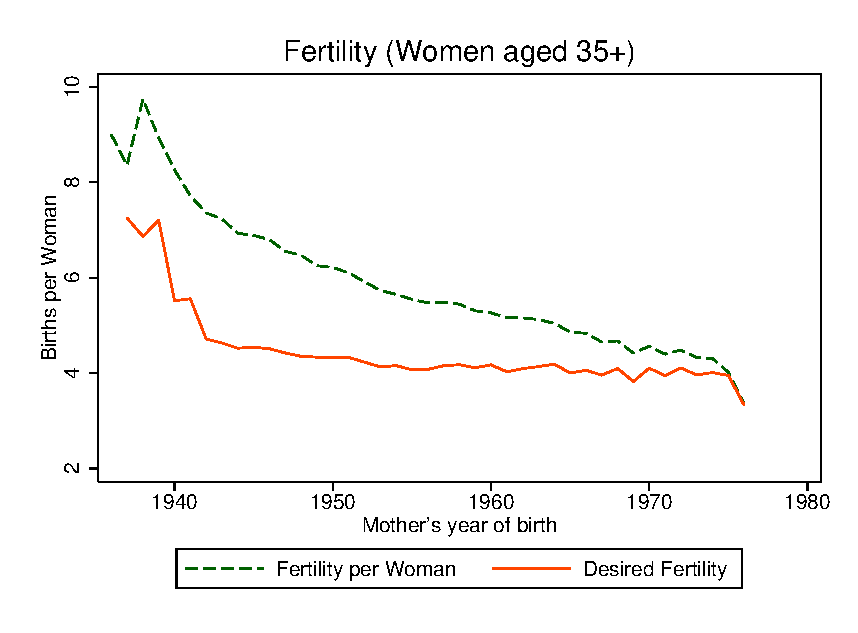
\includegraphics[scale=0.53]{\twinfolder/Figures/ferttrend_35_all.eps}
  \caption{Trends in Fertility}
  \label{TWINfig:fertrend}
\end{subfigure}%
\begin{subfigure}{.5\textwidth}
  \centering
  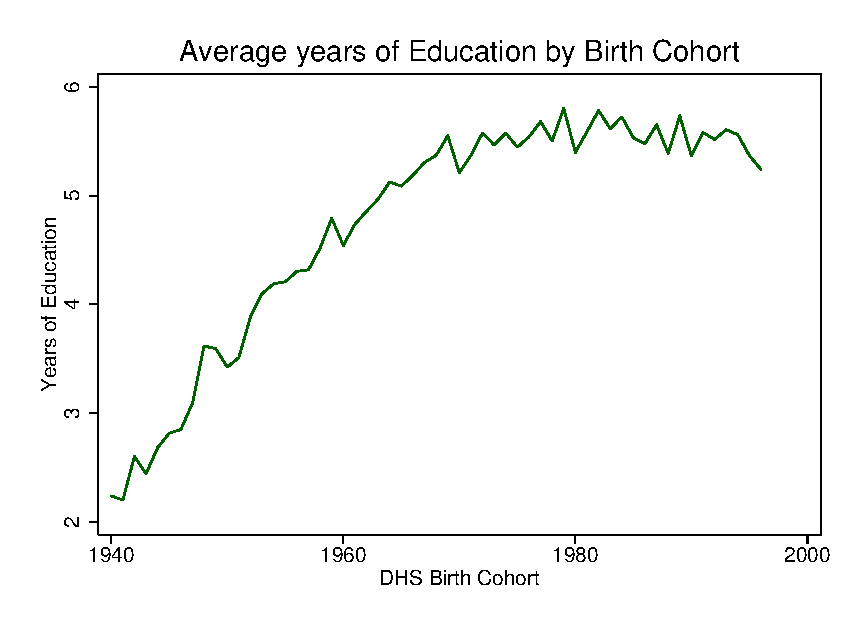
\includegraphics[scale=0.52]{\twinfolder/Figures/eductrend_all.eps}
  \caption{Trend in Education}
  \label{TWINfig:eductrend}
\end{subfigure}
\caption{Education and Fertility}
\label{TWINfig:trends}
\floatfoot{Note to figure \ref{TWINfig:trends}: Cohorts are made up of all individuals 
from the DHS who are over 35 years (for fertility), and over 15 years (for education).  
In each case the sample is restricted to those who have approximately completed fertility 
and education respectively.}
\end{figure}
\vspace{1cm}

\begin{figure}[htpb!]
\begin{center}
\caption{Proportion of Twins by Birth Order}
\label{TWINfig:bord}
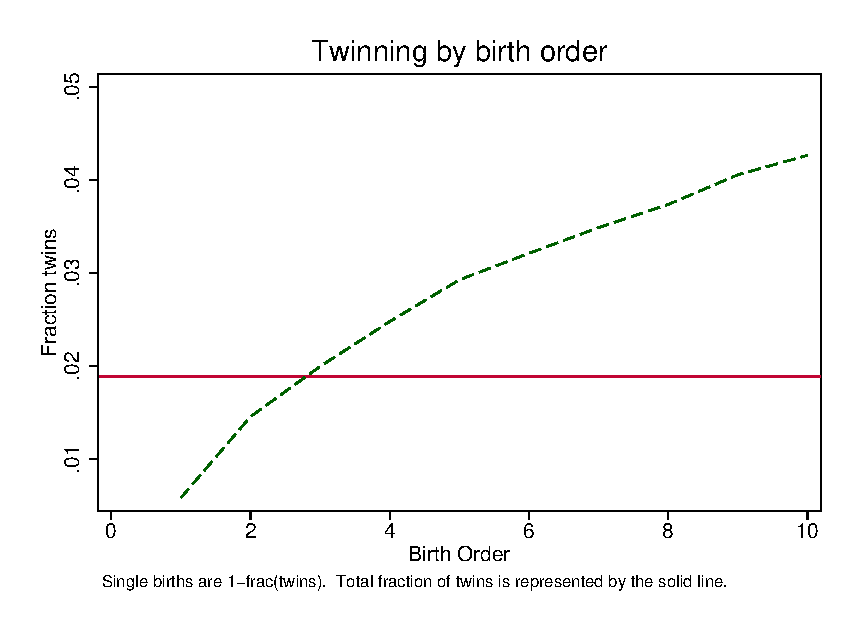
\includegraphics[scale=0.92]{\twinfolder/Figures/twinbybord.eps} 
\end{center}
\end{figure}

\begin{figure}[htpb!]
\begin{center}
\caption{Twin Births and Total Fertility}
\label{TWINfig:births}
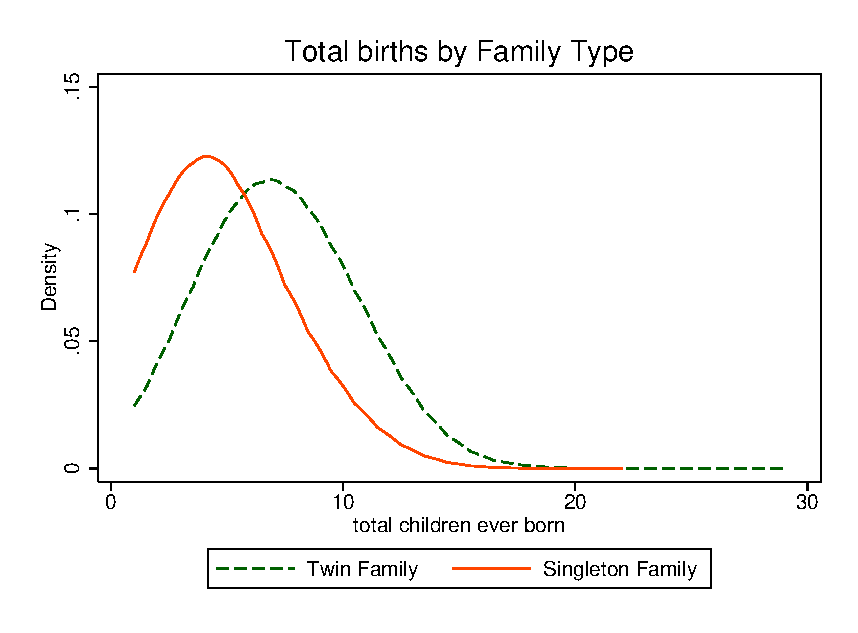
\includegraphics[scale=0.92]{\twinfolder/Figures/famsize.eps} 
\end{center}
\end{figure}

\begin{figure}[htpb!]
\begin{center}
\caption{Distribution of Ideal Family Size}
\label{TWINfig:ideal}
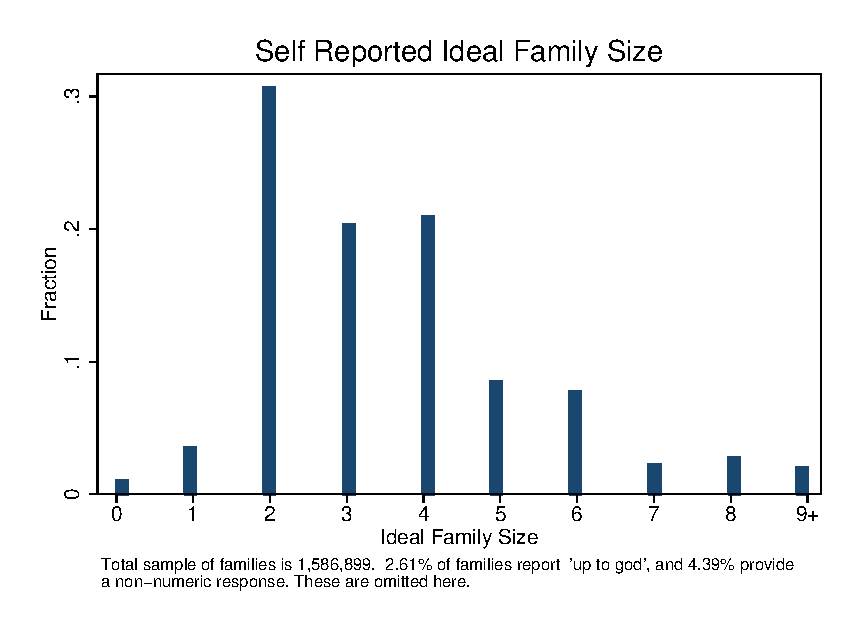
\includegraphics[scale=0.92]{\twinfolder/Figures/idealfamsize.eps} 
\end{center}
\end{figure}

\begin{figure}[htpb!]
\begin{center}
\caption{Ideal and Actual Fertility}
\label{TWINfig:idealactual}
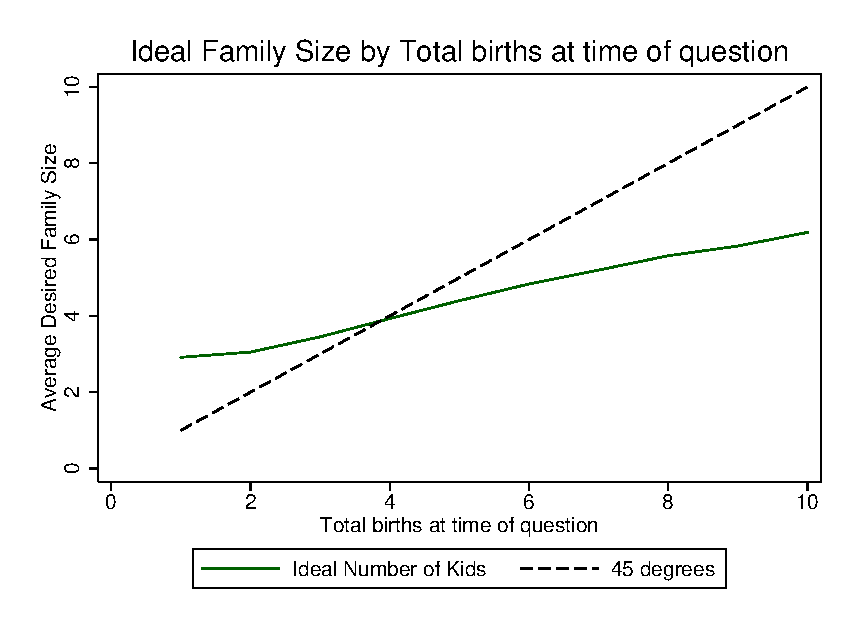
\includegraphics[scale=0.92]{\twinfolder/Figures/idealfam_fert.eps} 
\end{center}
\end{figure}

\begin{figure}[htpb!]
\begin{center}
\caption{Relaxing Strict Exogeneity (two plus)}
\label{TWINfig:ltz2}
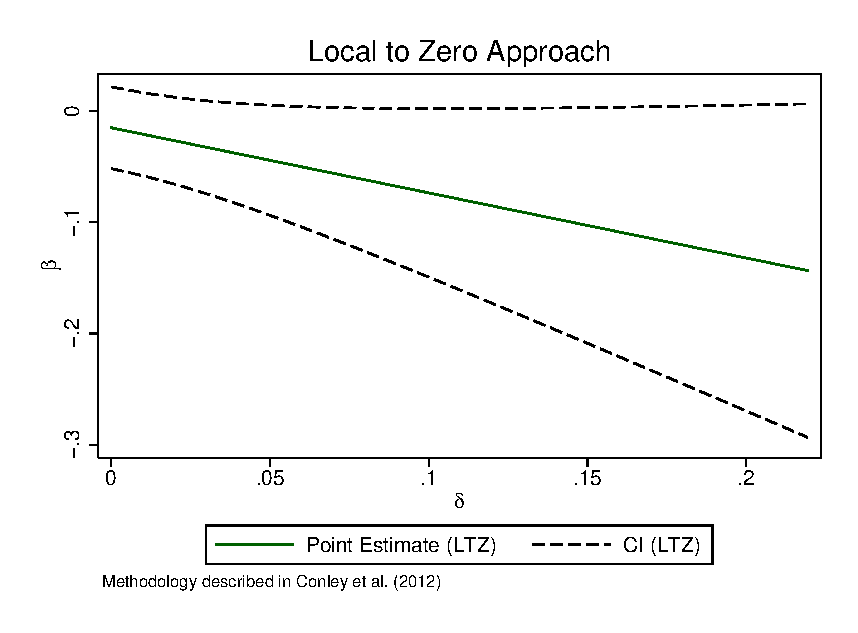
\includegraphics[scale=0.88]{\twinfolder/Figures/LTZ_two.eps}
\vspace{-8mm}
\floatfoot{Note to figure \ref{TWINfig:ltz2}: See note to Figure \ref{TWINfig:ltz3}}
\end{center}
\end{figure}

\begin{figure}[htpb!]
\begin{center}
\caption{Relaxing Strict Exogeneity (three plus)}
\label{TWINfig:ltz3}
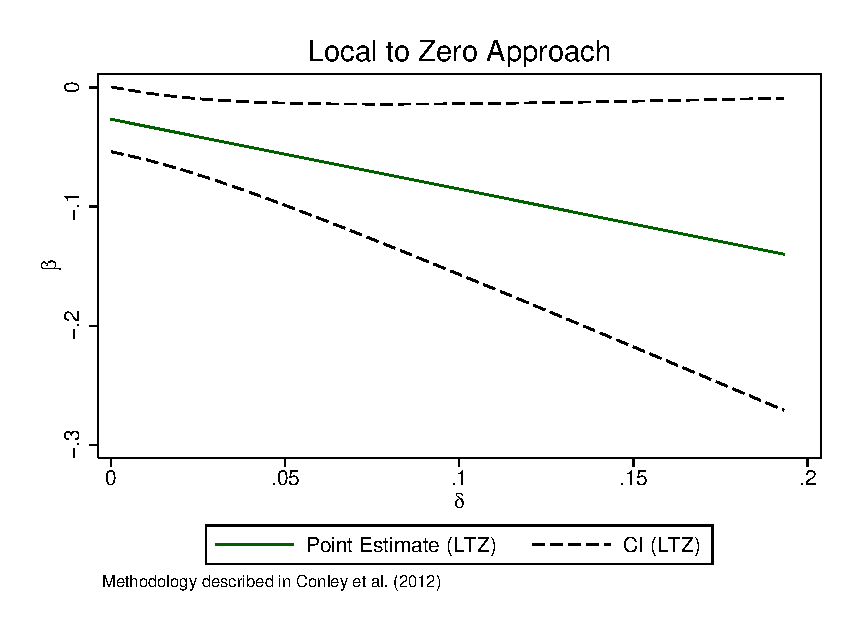
\includegraphics[scale=0.88]{\twinfolder/Figures/LTZ_three.eps} 
\floatfoot{Note to figure \ref{TWINfig:ltz3}: Confidence intervals and point estimates 
are calculated according to \citet{Conleyetal2012}.  Estimates reflect a range of priors 
regarding the validity of the exclusion restriction required to consistently estimate 
$\hat\beta_{fert}$ using twinning in a 2SLS framework.  The local to zero (LTZ) 
approach applied here assumes that $\gamma$, the sign on the instrument when included
in the first stage, is distributed $\gamma\sim U(0,\delta)$.  Further discussion 
is provided in the body of the text and table \ref{TWINtab:Conley}.}
\end{center}
\end{figure}

\clearpage

\section*{Tables}
\begin{table}[htpb!]\caption{Summary Statistics} 
\label{TWINtab:sumstats}\begin{center}\scalebox{0.99}{\begin{tabular}{lccccc}
\toprule \toprule 
&\multicolumn{2}{c}{Low Income}&\multicolumn{2}{c}{Middle Income}\\ 
\cmidrule(r){2-3} \cmidrule(r){4-5}
& Single & Twins & Single & Twins & All \\ \midrule 
\textsc{Fertility} & & & & & \\ 
Fertility&3.749&6.223&3.412&5.584&3.689\\
&(2.392)&(2.622)&(2.308)&(2.687)&(2.406)\\
Desired Family Size&4.193&5.328&3.380&4.190&3.921\\
&(2.530)&(2.885)&(2.130)&(2.555)&(2.440)\\
Fraction Twin & \multicolumn{2}{c}{  0.0200}& \multicolumn{2}{c}{  0.0179 } &  0.0191\\
& \multicolumn{2}{c}{(0.1402)}& \multicolumn{2}{c}{(0.1326)} & (0.1370)\\
Birth Order Twin & \multicolumn{2}{c}{   4.664}& \multicolumn{2}{c}{   4.016 }&   4.410\\
& \multicolumn{2}{c}{(2.465)}& \multicolumn{2}{c}{(2.374)}& (2.450)\\
\textsc{Mother's Characteristics}&&&&&\\ Age
&31.22&34.52&32.32&35.61&31.72\\
&(8.238)&(7.381)&(8.356)&(7.428)&(8.293)\\
Education&3.859&3.222&6.690&5.906&4.885\\
&(4.327)&(3.991)&(4.795)&(5.023)&(4.706)\\
Height&155.5&157.6&155.6&157.2&155.6\\
&(7.093)&(7.065)&(6.966)&(6.945)&(7.053)\\
BMI&21.90&22.50&25.90&26.63&23.39\\
&(4.027)&(4.175)&(5.118)&(5.512)&(4.867)\\
Pr(BMI)$<$18.5&0.175&0.125&0.0346&0.0276&0.122\\
&(0.380)&(0.331)&(0.183)&(0.164)&(0.327)\\
Actual Births$>$Desired&0.310&0.526&0.324&0.575&0.321\\
&(0.463)&(0.499)&(0.468)&(0.494)&(0.467)\\
\textsc{Children's Outcomes}&&&&&\\ Education (Years)
&3.660&3.204&5.445&5.043&4.446\\
&(3.576)&(3.293)&(3.867)&(3.760)&(3.810)\\
Education (Z-Score)&-0.00843&-0.0156&0.0119&-0.0428&0.000144\\
&(1.001)&(0.963)&(0.998)&(0.987)&(1.000)\\
No Education (Percent)&0.207&0.222&0.0649&0.0786&0.144\\
&(0.405)&(0.416)&(0.246)&(0.269)&(0.351)\\
Infant Mortality&0.0158&0.0917&0.00946&0.0497&0.0141\\
&(0.125)&(0.289)&(0.0968)&(0.217)&(0.118)\\
Child Mortality&0.0239&0.108&0.0122&0.0535&0.0199\\
&(0.153)&(0.310)&(0.110)&(0.225)&(0.140)\\
\midrule
Number of Countries & 39&39  & 28&28  & 67 \\
Number of Children &2,231,844 &45,654 &1,614,358 &29,430 & 3,921,286 \\
Number of Mothers &875,587 &12,908 &653,969 &8,605 & 1,586,899 \\
\midrule
\multicolumn{6}{p{13.2cm}}{\begin{footnotesize}\textsc{Notes:}  Group means are presented with standard deviation below in parenthesis.  Education is reported as total years attained, and Z-score presents educational attainment relative to country and cohort (mean 0, std deviation 1).  Infant mortality refers to the proportion of children who die before 1 year of age,  while child mortality refers to the proportion who die before 5 years.  Maternal height is reported in cm, and BMI is weight in kg over height in metres squared.  Summary statistics are for the full sample of 1,586,899
 mothers responding to any publicly available DHS survey.  For a full list of country and years of survey, see appendix table \ref{TWINtab:countries}.\end{footnotesize}} \\ \bottomrule \end{tabular}}\end{center}\end{table}

\begin{table}[htbp]\centering
\def\sym#1{\ifmmode^{#1}\else\(^{#1}\)\fi}
\caption{Test of Balance of Observables: Twins versus Non-twins \label{TWINtab:comp}}
\vspace{5mm}\begin{tabular}{l*{1}{ccc}}
\toprule\toprule & Non-Twin & Twin & Diff.\\
                    &        Family&        Family&      (Diff. SE)         \\
\midrule
Total Fertilty      &       4.460&       6.787&      -2.327\sym{***}\\
                    &            &            &    (0.0255)         \\
Desired Fertility   &       4.451&       5.566&      -1.116\sym{***}\\
                    &            &            &    (0.0312)         \\
Age First Birth     &       19.15&       18.98&       0.170\sym{***}\\
                    &            &            &    (0.0424)         \\
Mother's Education  &       4.269&       3.351&       0.918\sym{***}\\
                    &            &            &    (0.0523)         \\
Father's Education  &       5.510&       4.710&       0.800\sym{***}\\
                    &            &            &    (0.0584)         \\
Mother's Height     &       156.1&       157.8&      -1.716\sym{***}\\
                    &            &            &    (0.0839)         \\
Pr(BMI $<$ 18.5)    &       0.120&      0.0937&      0.0265\sym{***}\\
                    &            &            &   (0.00382)         \\
Number of Antenatal Checks&       3.901&       3.815&      0.0860\sym{*}  \\
                    &            &            &    (0.0374)         \\
Prenatal care (doctor)&       0.313&       0.211&       0.102\sym{***}\\
                    &            &            &   (0.00544)         \\
Prenatal care (nurse)&       0.452&       0.521&     -0.0690\sym{***}\\
                    &            &            &   (0.00588)         \\
Prenatal care (none)&       0.193&       0.183&     0.00979\sym{*}  \\
                    &            &            &   (0.00466)         \\
Mother's Age        &       25.53&       27.61&      -2.077\sym{***}\\
                    &            &            &    (0.0565)         \\
Child Mortality     &      0.0102&      0.0255&     -0.0153\sym{***}\\
                    &            &            &  (0.000912)         \\
Infant Mortality    &     0.00580&      0.0170&     -0.0112\sym{***}\\
                    &            &            &  (0.000606)         \\
Wealth Quintile 1   &       0.259&       0.274&     -0.0154\sym{**} \\
                    &            &            &   (0.00518)         \\
Wealth Quintile 2   &       0.220&       0.227&    -0.00691         \\
                    &            &            &   (0.00490)         \\
Wealth Quintile 3   &       0.198&       0.201&    -0.00351         \\
                    &            &            &   (0.00471)         \\
Wealth Quintile 4   &       0.176&       0.175&    0.000653         \\
                    &            &            &   (0.00450)         \\
Wealth Quintile 5   &       0.148&       0.123&      0.0252\sym{***}\\
                    &            &            &   (0.00418)         \\
\midrule\midrule


\multicolumn{4}{p{10.4cm}}{\begin{footnotesize}\textsc{Notes:} Education measured in years, mother's height in centimetres, and BMI is weight in kilograms over height in metres squared.  Diff. SE is calculated using a two-tailed t-test. $^{*}$p$<$0.1; $^{**}$p$<$0.05; $^{***}$p$<$0.01\end{footnotesize}}
\\\bottomrule\normalsize\end{tabular}\end{table} 


\begin{table}[htpb!]
\caption{Test of hypothesis that women who bear twins have better prior health}\label{TWINtab:IMR}\begin{center}\begin{tabular}{lccc}
\toprule \toprule 
\textsc{Infant Mortality (per 100 births)}& Base & +S\&H & Observations \\ \midrule 
\begin{footnotesize}\end{footnotesize}& 
\begin{footnotesize}\end{footnotesize}& 
\begin{footnotesize}\end{footnotesize}& 
\begin{footnotesize}\end{footnotesize}\\ 
Treated (2+)\hspace{5mm}\hspace{5mm}\hspace{5mm}\hspace{5mm}\hspace{5mm}\hspace{5mm}&-2.065***&-2.110***&503785\\
&(0.212)&(0.213)&\\
Treated (3+)\hspace{5mm}&-4.619***&-4.632***&686931\\
&(0.201)&(0.201)&\\
Treated (4+)&-4.257***&-4.243***&676303\\
&(0.183)&(0.183)&\\
Treated (5+)&-3.353***&-3.324***&587919\\
&(0.183)&(0.183)&\\
\midrule\multicolumn{4}{p{12.1cm}}{\begin{footnotesize}\textsc{Notes:} The sample for these regressions consist of all children who have been entirely exposed to the risk of infant mortality (ie those over 1 year of age). Subsamples 2+, 3+, 4+ and 5+ are generated to allow comparison of children born at similar birth orders.  For a full description of these groups see the the body of the paper or notes to table \ref{TWINtab:IVAll}. Treated=1 refers to children who are born before a twin while Treated=0 refers to children of similar birth orders not born before a twin.  Base and S+H controls are described in table \ref{TWINtab:IVAll}.$^{*}$p$<$0.1; $^{**}$p$<$0.05; $^{***}$p$<$0.01 
\end{footnotesize}} \\ \bottomrule 
\end{tabular}\end{center}\end{table}

\begin{landscape}\begin{table}[!htbp] \centering 
\caption{OLS Estimates of the Q-Q Trade-off} 
 \vspace{4mm}\label{TWINtab:OLS} 
\begin{tabular}{lcccccc} \toprule \toprule 
&Base&+&+&Desired&Altonji&Altonji\\
&Controls&Socioec&Health&&Ratio 1&Ratio 2\\\midrule
\textsc{Panel A: All Countries}&&&&&&\\
Fertility &-0.115***&-0.0777***&-0.0751***&-0.0717***&2.083&1.882\\
&(0.000815)&(0.000776)&(0.000771)&(0.000838)&&\\
Fertility$\times$desire&&&&-0.00558***&&\\
&&&&(0.000495)&&\\
&&&&&&\\
Observations &1,334,874&1,334,874&1,334,874&1,334,874&&\\
R$^2$&0.094&0.161&0.167&0.168&&\\\midrule
\textsc{Panel B: Low Income}&&&&&&\\
Fertility &-0.110***&-0.0734***&-0.0712***&-0.0668***&2.005&1.835\\
&(0.00106)&(0.000988)&(0.000975)&(0.00107)&&\\
Fertility$\times$desire&&&&-0.00674***&&\\
&&&&(0.000608)&&\\
&&&&&&\\
Observations &831,476&831,476&831,476&831,476&&\\
R$^2$&0.091&0.171&0.181&0.182&&\\\midrule
\textsc{Panel C: Middle Income}&&&&&&\\
Fertility &-0.125***&-0.0875***&-0.0854***&-0.0839***&2.333&2.157\\
&(0.00128)&(0.00126)&(0.00126)&(0.00134)&&\\
Fertility$\times$desire&&&&-0.00266***&&\\
&&&&(0.000846)&&\\
&&&&&&\\
Observations &503,398&503,398&503,398&503,398&&\\
R$^2$&0.106&0.154&0.156&0.156&&\\\hline\hline
\multicolumn{7}{p{15.8cm}}{\begin{footnotesize}\textsc{Notes:} Base controls consist of child gender, mother's age and age squared mother's age at first birth, child age, country, and year of birth dummies.  Socioeconomic augments `Base' to include mother's education and education squared, and Health includes mother's height and BMI. ``Desire'' takes 1 if the child is born before the family reaches it's desired size, and 0 if the child is born after the desired size is reached. The \citet{Altonjietal2005} ratio determines how important unobservable factors must be compared with included observables to imply that the true effect of fertilty on educational attainment is equal to zero.  Ratio 1 compares no controls to socioeconomic controls, while ratio 2 compares no controls to socioeconomic and health controls. Standard errors are clustered at the level of the mother.
$^{*}$p$<$0.1; $^{**}$p$<$0.05; $^{***}$p$<$0.01\end{footnotesize}}\\  
\bottomrule \normalsize\end{tabular}\end{table}\end{landscape} 


\begin{table}[!htbp] \centering 
\caption{Instrumental Variables Estimates: Two Plus} 
\label{TWINtab:IVTwoplus} 
\begin{tabular}{lcccc} \toprule \toprule 
&Base&&&\\
&Controls&Socioec&Health&Obs.\\\midrule
\multicolumn{5}{l}{\textsc{Pre-Twins}}\\ 
&&&&\\
\multicolumn{5}{l}{\textbf{All Families}}\\ 
Fertility&0.006&-0.026&-0.026&249,536\\
         &(0.029)&(0.027)&(0.026)&\\
&&&&\\
\multicolumn{5}{l}{\textbf{Low-Income Countries}}\\ 
Fertility&0.035&0.008&0.012&149,602\\
         &(0.034)&(0.032)&(0.031)&\\
&&&&\\
\multicolumn{5}{l}{\textbf{Middle-Income Countries}}\\ 
Fertility&-0.065&-0.087*&-0.093**&99,934\\
         &(0.053)&(0.049)&(0.047)&\\
&&&&\\
\multicolumn{5}{l}{\textbf{Desired-Threshold}}\\ 
Fertility&0.007&-0.025&-0.027&249,536\\
         &(0.035)&(0.031)&(0.030)&\\
Fertility$\times$desire&-0.001&0.001&0.000&\\
         &(0.014)&(0.013)&(0.013)&\\
\midrule\multicolumn{5}{l}{\textsc{Twins and Pre-Twins}}\\ 
&&&&\\
\multicolumn{5}{l}{\textbf{All Families}}\\ 
Fertility&-0.021&-0.073***&-0.078***&488,815\\
         &(0.024)&(0.021)&(0.020)&\\
\midrule\multicolumn{5}{l}{\textsc{First Stage (Pre-Twins)}}\\ 
&&&&\\
\multicolumn{5}{l}{\textbf{All Families}}\\ 
Twins&0.776***&0.821***&0.822***&249,536\\
         &(0.031)&(0.029)&(0.028)&\\
\hline\multicolumn{5}{p{10.0cm}}{\begin{footnotesize}\textsc{Notes:} Two-plus refers to all first-born children in families with two or more children.  Each cell presents the coefficient of a 2SLS regression where fertility is instrumented by twinning at birth order two.  Base controls include child age, mother's age, and mother's age at birth fixed effects plus country and year-of-birth FEs.  The sample is made up of all children aged between 6-18 years from families in the DHS who fulfill two-plus requirements. First-stage results in the final panel correspond to the second stage in row 1.  Full first stage results for each row are available in table \ref{TWINtab:FS}. Standard errors are clustered by mother. 
$^{*}$p$<$0.1; $^{**}$p$<$0.05; $^{***}$p$<$0.01\end{footnotesize}}
\\\bottomrule\normalsize\end{tabular}\end{table} 


\begin{table}[!htbp] \centering 
\caption{Instrumental Variables Estimates: Three Plus} 
\label{TWINtab:IVThreeplus} 
\begin{tabular}{lcccc} \toprule \toprule 
&Base&&&\\
&Controls&Socioec&Health&Obs.\\\midrule
\multicolumn{5}{l}{\textsc{Pre-Twins}}\\ 
&&&&\\
\multicolumn{5}{l}{\textbf{All Families}}\\ 
Fertility&-0.010&-0.038*&-0.042**&390,985\\
         &(0.023)&(0.021)&(0.021)&\\
&&&&\\
\multicolumn{5}{l}{\textbf{All Families (bord dummies)}}\\ 
Fertility&-0.010&-0.038*&-0.042**&390,985\\
         &(0.023)&(0.021)&(0.020)&\\
&&&&\\
\multicolumn{5}{l}{\textbf{Low-Income Countries}}\\ 
Fertility&0.006&-0.029&-0.034&244,928\\
         &(0.029)&(0.026)&(0.025)&\\
&&&&\\
\multicolumn{5}{l}{\textbf{Middle-Income Countries}}\\ 
Fertility&-0.045&-0.061*&-0.064*&146,057\\
         &(0.039)&(0.035)&(0.035)&\\
&&&&\\
\multicolumn{5}{l}{\textbf{Desired-Threshold}}\\ 
Fertility&0.001&-0.044*&-0.047**&390,985\\
         &(0.027)&(0.024)&(0.024)&\\
Fertility$\times$desire&-0.011&0.002&0.001&\\
         &(0.010)&(0.009)&(0.009)&\\
\midrule\multicolumn{5}{l}{\textsc{Twins and Pre-Twins}}\\ 
&&&&\\
\multicolumn{5}{l}{\textbf{All Families}}\\ 
Fertility&-0.025&-0.066***&-0.071***&584,566\\
         &(0.020)&(0.018)&(0.018)&\\
&&&&\\
\multicolumn{5}{l}{\textbf{All Families (bord dummies)}}\\ 
Fertility&-0.020&-0.054***&-0.058***&584,566\\
         &(0.021)&(0.019)&(0.018)&\\
\midrule\multicolumn{5}{l}{\textsc{First Stage (Pre-Twins)}}\\ 
&&&&\\
\multicolumn{5}{l}{\textbf{All Families}}\\ 
Twins&0.796***&0.821***&0.824***&390,985\\
         &(0.027)&(0.026)&(0.026)&\\
\hline\multicolumn{5}{p{10cm}}{\begin{footnotesize}\textsc{Notes:} Three-plus refers to all first- and second-born children in families with three or more children.  Each cell presents the coefficient of a 2SLS regression where fertility is instrumented by twinning at birth order three.  Base controls include child age, mother's age, and mother's age at birth fixed effects plus country and year-of-birth FEs.  The sample is made up of all children aged between 6-18 years from families in the DHS who fulfill three-plus requirements. Birth order dummies are included only if explicitly stated.  First-stage results in the final panel correspond to the second stage in row 1.  Full first stage results for each row are available in table \ref{TWINtab:FS}. Standard errors are clustered by mother. 
$^{*}$p$<$0.1; $^{**}$p$<$0.05; $^{***}$p$<$0.01\end{footnotesize}}
\\\bottomrule\normalsize\end{tabular}\end{table} 


\begin{table}[!htbp] \centering 
\caption{Instrumental Variables Estimates: Four Plus} 
\label{TWINtab:IVFourplus} 
\begin{tabular}{lcccc} \toprule \toprule 
&Base&&&\\
&Controls&Socioec&Health&Obs.\\\midrule
\multicolumn{5}{l}{\textsc{Pre-Twins}}\\ 
&&&&\\
\multicolumn{5}{l}{\textbf{All Families}}\\ 
Fertility&-0.017&-0.036&-0.035*&385,389\\
         &(0.025)&(0.023)&(0.021)&\\
&&&&\\
\multicolumn{5}{l}{\textbf{Low-Income Countries}}\\ 
Fertility&-0.011&-0.031&-0.024&246,622\\
         &(0.029)&(0.027)&(0.025)&\\
&&&&\\
\multicolumn{5}{l}{\textbf{Middle-Income Countries}}\\ 
Fertility&-0.027&-0.048&-0.054&138,767\\
         &(0.043)&(0.040)&(0.037)&\\
&&&&\\
\multicolumn{5}{l}{\textbf{Desired-Threshold}}\\ 
Fertility&-0.003&-0.017&-0.020&385,389\\
         &(0.027)&(0.023)&(0.023)&\\
Fertility$\times$desire&-0.012&-0.012&-0.013*&\\
         &(0.008)&(0.007)&(0.007)&\\
\midrule\multicolumn{5}{l}{\textsc{Twins and Pre-Twins}}\\ 
&&&&\\
\multicolumn{5}{l}{\textbf{All Families}}\\ 
Fertility&-0.018&-0.039**&-0.046**&523,197\\
         &(0.021)&(0.019)&(0.018)&\\
\midrule\multicolumn{5}{l}{\textsc{First Stage (Pre-Twins)}}\\ 
&&&&\\
\multicolumn{5}{l}{\textbf{All Families}}\\ 
Twins&0.840***&0.859***&0.861***&385,389\\
         &(0.027)&(0.027)&(0.026)&\\
\hline\multicolumn{5}{p{10.0cm}}{\begin{footnotesize}\textsc{Notes:} Four-plus refers to all first- to third-born children in families with four or more children.  Each cell presents the coefficient of a 2SLS regression where fertility is instrumented by twinning at birth order four.  Base controls include child age, mother's age, and mother's age at birth fixed effects plus country and year-of-birth FEs.  The sample is made up of all children aged between 6-18 years from families in the DHS who fulfill four-plus requirements. First-stage results in the final panel correspond to the second stage in row 1.  Full first stage results for each row are available in table \ref{TWINtab:FS}. Standard errors are clustered by mother. 
$^{*}$p$<$0.1; $^{**}$p$<$0.05; $^{***}$p$<$0.01\end{footnotesize}}
\\\bottomrule\normalsize\end{tabular}\end{table} 


\begin{table}[htpb!]\caption{`Plausibly Exogenous' Bounds} 
\label{TWINtab:Conley}\begin{center}\begin{tabular}{lcccc}
\toprule \toprule 
&\multicolumn{2}{c}{UCI: $\gamma\in [0,\delta]$}&\multicolumn{2}{c}{LTZ: $\gamma \sim U(0,\delta)$}\\ 
\cmidrule(r){2-3} \cmidrule(r){4-5}
&Lower Bound&Upper Bound&Lower Bound&Upper Bound\\
Two Plus&-0.1860&0.0195&-0.1613&0.0011\\
Three Plus&-0.1710&0.0025&-0.1528&-0.0116\\
Four Plus&-0.1539&-0.0067&-0.1391&-0.0194\\
Five Plus&-0.1373&0.0277&-0.1215&0.0143\\
\midrule\multicolumn{5}{p{11.6cm}}{\begin{footnotesize}\textsc{Notes:} This table presents upper and lower bounds of a 95\% confidence interval for the effects of family size on (standardised) children's education attainment. These are estimated by the methodology of \citet{Conleyetal2012}  under various priors about the direct effect that being from a twin family has on educational outcomes ($\gamma$). In the UCI (union of confidence interval) approach, it is assumed the true $\gamma\in[0,\delta]$, while in the LTZ (local to zero) approach it is assumed that $\gamma\sim U(0,\delta)$.  In each case $\delta$ is estimated by including twinning in the first stage  equation and observing the effect size $\hat\gamma$.  Estimated $\hat\gamma$'s are (respectively for two plus to five plus):   0.1088, 0.0983, 0.0826, 0.0929.\end{footnotesize}}  
\\ \bottomrule \end{tabular}\end{center}\end{table} 


\begin{table}[htpb!]\caption{Q-Q IV Estimates by Gender} 
\label{TWINtab:gend}\begin{center}\begin{tabular}{lcccccccc}
\toprule \toprule 
&\multicolumn{4}{c}{Females}&\multicolumn{4}{c}{Males}\\ 
\cmidrule(r){2-5} \cmidrule(r){6-9} 
&Base&Socioec&Health&Obs.&Base&Socioec&Health&Obs. \\ \midrule 
\begin{footnotesize}\end{footnotesize}&\begin{footnotesize}\end{footnotesize}&\begin{footnotesize}\end{footnotesize}&\begin{footnotesize}\end{footnotesize}&\begin{footnotesize}\end{footnotesize}&\begin{footnotesize}\end{footnotesize}&\\Two Plus &0.005&-0.039&-0.037&122,414&0.010&-0.010&-0.015&127,122\\
&(0.043)&(0.039)&(0.038)&&(0.040)&(0.038)&(0.036)&\\
\begin{footnotesize}\end{footnotesize}&\begin{footnotesize}\end{footnotesize}&\begin{footnotesize}\end{footnotesize}&\begin{footnotesize}\end{footnotesize}&\begin{footnotesize}\end{footnotesize}&\begin{footnotesize}\end{footnotesize}&\\Three Plus &-0.024&-0.056*&-0.052*&187,098&0.016&-0.015&-0.022&188,889\\
&(0.033)&(0.030)&(0.029)&&(0.030)&(0.028)&(0.027)&\\
\begin{footnotesize}\end{footnotesize}&\begin{footnotesize}\end{footnotesize}&\begin{footnotesize}\end{footnotesize}&\begin{footnotesize}\end{footnotesize}&\begin{footnotesize}\end{footnotesize}&\begin{footnotesize}\end{footnotesize}&\\Four Plus &-0.029&-0.052*&-0.053**&192,714&-0.005&-0.020&-0.018&192,675\\
&(0.032)&(0.029)&(0.027)&&(0.030)&(0.028)&(0.027)&\\
\midrule\multicolumn{9}{p{14.2cm}}{\begin{footnotesize}\textsc{Notes:} Female or male refers to the gender of the index child of the regression. 
All regressions include full controls including socioeconomic and maternal health variables.  The full lis of controls are available in 
the notes to table \ref{TWINtab:IVAll}.  Full IV results for male and female children are presented in table \ref{TWINtab:IVgend}. Standard errors are clustered 
 by mother.$^{*}$p$<$0.1; $^{**}$p$<$0.05; $^{***}$p$<$0.01
\end{footnotesize}} \\ \bottomrule 
\end{tabular}\end{center}\end{table}

\clearpage
\newpage

\bibliography{./BiBBase1}

\newpage
\appendix
\section*{Appendices}

\section{Appendix Tables}
%\begin{table}[htpb!]
\caption{Desired Fertility and Observable Characteristics}
\begin{tabular}{lccc} \hline\hline
& Desired & Shortfall & Twin \\
& fertility & & threshold \\ \hline
\vspace{4pt} & \begin{footnotesize}\end{footnotesize} & \begin{footnotesize}\end{footnotesize} & \begin{footnotesize}\end{footnotesize} \\
Mother's Age & 0.0700*** & 0.255*** & 0.0869  \\
\vspace{4pt} & \begin{footnotesize}(0.00263)\end{footnotesize} & \begin{footnotesize}(0.00304)\end{footnotesize} & \begin{footnotesize}(0.115)\end{footnotesize} \\
Mother's Age Squared & -0.000129*** & -0.000802*** & -0.00560*** \\
\vspace{4pt} & \begin{footnotesize}(5.00e-05)\end{footnotesize} & \begin{footnotesize}(5.74e-05)\end{footnotesize} & \begin{footnotesize}(0.00193)\end{footnotesize} \\
Age First Birth & -0.0674*** & -0.236*** & 0.246*** \\
\vspace{4pt} & \begin{footnotesize}(0.00105)\end{footnotesize} & \begin{footnotesize}(0.00122)\end{footnotesize} & \begin{footnotesize}(0.0515)\end{footnotesize} \\
Mother's Education & -0.157*** & 0.0345*** & 0.391*** \\
\vspace{4pt} & \begin{footnotesize}(0.00202)\end{footnotesize} & \begin{footnotesize}(0.00237)\end{footnotesize} & \begin{footnotesize}(0.149)\end{footnotesize} \\
Mother's Education Squared & 0.00613*** & -0.00407*** & 0.0112 \\
\vspace{4pt} & \begin{footnotesize}(0.000139)\end{footnotesize} & \begin{footnotesize}(0.000162)\end{footnotesize} & \begin{footnotesize}(0.0131)\end{footnotesize} \\
Height & 0.000363 & 0.000128 & -1.10e-05 \\
\vspace{4pt} & \begin{footnotesize}(0.000542)\end{footnotesize} & \begin{footnotesize}(0.000625)\end{footnotesize} & \begin{footnotesize}(0.0293)\end{footnotesize} \\
BMI & -0.0129*** & 0.0136*** & 0.108** \\
\vspace{4pt} & \begin{footnotesize}(0.000789)\end{footnotesize} & \begin{footnotesize}(0.000908)\end{footnotesize} & \begin{footnotesize}(0.0475)\end{footnotesize} \\
Constant & 4.996*** & 4.389*** & 1.580 \\
 & \begin{footnotesize}(0.0975)\end{footnotesize} & \begin{footnotesize}(0.114)\end{footnotesize}&\begin{footnotesize}(6.575)\end{footnotesize} \\
\vspace{4pt} & \begin{footnotesize}\end{footnotesize} & \begin{footnotesize}\end{footnotesize} \\
Observations & 2,086,040 & 2,086,040 & 138,014 \\
 $R^2$ & 0.457 & 0.384 & 0.052 \\ \hline
\multicolumn{4}{p{11.2cm}}{\begin{footnotesize} \textsc{Notes:}  All regressions are at the level of the mother.  Desired fertility is total number 
of births reported by mother as desired at the time of the survey.  Shortfall represents the difference between total desired fertility and actual 
births.  Twin threshold takes the value of 1 if twins in a twin family cause families to exceed their total desired fertility, and 0 if twins do 
not cause families to exceed their desired fertility. *** p$<$0.01, ** p$<$0.05, * p$<$0.1\end{footnotesize}} \\ \hline
\end{tabular}
\end{table}
\newpage


\end{spacing}\begin{spacing}{1} 
\begin{longtable}{llccccccc}\caption{Full Survey Countries and Years} \\ 
\toprule\label{TWINtab:countries} 
& & \multicolumn{7}{c}{Survey Year} \\ \cmidrule(r){3-9} 
\textsc{Country}&\textsc{Income}&1&2&3&4&5&6&7\\ \midrule 
Albania&Middle&2008&&&&&&\\
Armenia&Low&2000&2005&2010&&&&\\
Azerbaijan&Middle&2006&&&&&&\\
Bangladesh&Low&1994&1997&2000&2004&2007&2011&\\
Benin&Low&1996&2001&2006&&&&\\
Bolivia&Middle&1989&1994&1998&2003&2008&&\\
Brazil&Middle&1986&1991&1996&&&&\\
Burkina Faso&Low&1993&1999&2003&2010&&&\\
Burundi&Low&1987&2010&&&&&\\
Cambodia&Low&2000&2005&2010&&&&\\
Cameroon&Middle&1991&1998&2004&2011&&&\\
Central African Republic&Low&1994&&&&&&\\
Chad&Low&1997&2004&&&&&\\
Colombia&Middle&1986&1990&1995&2000&2005&2010&\\
Comoros&Low&1996&&&&&&\\
Congo Brazzaville&Middle&2005&2011&&&&&\\
Congo, Dem&Low&2007&&&&&&\\
Cote d'Ivoire&Low&1994&1998&2005&2012&&&\\
Dominican Republic&Middle&1986&1991&1996&1999&2002&2007&\\
Ecuador&Middle&1987&&&&&&\\
Egypt, Arab Rep&Middle&1988&1992&1995&2000&2005&2008&\\
El Salvador&Middle&1985&&&&&&\\
Ethiopia&Low&2000&2005&2011&&&&\\
Gabon&Middle&2000&2012&&&&&\\
Ghana&Low&1988&1993&1998&2003&2008&&\\
Guatemala&Middle&1987&1995&&&&&\\
Guinea&Low&1999&2005&&&&&\\
Guyana&Middle&2005&2009&&&&&\\
Haiti&Low&1994&2000&2006&2012&&&\\
Honduras&Middle&2005&2011&&&&&\\
India&Low&1993&1999&2006&&&&\\
Indonesia&Low&1987&1991&1994&1997&2003&2007&2012\\
Jordan&Middle&1990&1997&2002&2007&&&\\
Kazakhstan&Middle&1995&1999&&&&&\\
Kenya&Low&1989&1993&1998&2003&2008&&\\
Kyrgyz Republic&Low&1997&&&&&&\\
Lesotho&Low&2004&2009&&&&&\\
Liberia&Low&1986&2007&&&&&\\
Madagascar&Low&1992&1997&2004&2008&&&\\
Malawi&Low&1992&2000&2004&2010&&&\\
Maldives&Middle&2009&&&&&&\\
Mali&Low&1987&1996&2001&2006&&&\\
Mexico&Middle&1987&&&&&&\\
Moldova&Middle&2005&&&&&&\\
Morocco&Middle&1987&1992&2003&&&&\\
Mozambique&Low&1997&2003&2011&&&&\\
Namibia&Middle&1992&2000&2006&&&&\\
Nepal&Low&1996&2001&2006&2011&&&\\
Nicaragua&Low&1998&2001&&&&&\\
Niger&Low&1992&1998&2006&&&&\\
Nigeria&Low&1990&1999&2003&2008&&&\\
Pakistan&Low&1991&2006&&&&&\\
Paraguay&Middle&1990&&&&&&\\
Peru&Middle&1986&1992&1996&2000&&&\\
Philippines&Middle&1993&1998&2003&2008&&&\\
Rwanda&Low&1992&2000&2005&2010&&&\\
Sao Tome and Principe&Middle&2008&&&&&&\\
Senegal&Low&1986&1993&1997&2005&2010&&\\
Sierra Leone&Low&2008&&&&&&\\
South Africa&Middle&1998&&&&&&\\
Sri Lanka&Low&1987&&&&&&\\
Sudan&Low&1990&&&&&&\\
Swaziland&Middle&2006&&&&&&\\
Tanzania&Low&1992&1996&1999&2004&2007&2010&2012\\
Thailand&Middle&1987&&&&&&\\
Togo&Low&1988&1998&&&&&\\
Trinidad and Tobago&Middle&1987&&&&&&\\
Tunisia&Middle&1988&&&&&&\\
Turkey&Middle&1993&1998&2003&&&&\\
Uganda&Low&1988&1995&2000&2006&2011&&\\
Ukraine&Middle&2007&&&&&&\\
Uzbekistan&Middle&1996&&&&&&\\
Vietnam&Low&1997&2002&&&&&\\
Yemen, Rep&Low&1991&&&&&&\\
Zambia&Low&1992&1996&2002&2007&&&\\
Zimbabwe&Middle&1988&1994&1999&2005&2010\\
\midrule\multicolumn{9}{p{13.3cm}}{\begin{footnotesize}\textsc{Notes:} Country income status is based upon World Bank classifications described at http://data.worldbank.org/about/country-classifications and available for download at http://siteresources.worldbank.org/DATASTATISTICS/Resources/OGHIST.xls (consulted 1 April, 2014).  Income status varies by country and time.  Where a country's status changed between DHS waves only the most recent status is listed above.  Middle refers to both lower-middle and upper-middle income countries, while low refers just to those considered to be low-income economies.\end{footnotesize}}  
\\ \bottomrule \end{longtable}\end{spacing}\begin{spacing}{1.5}

%\begin{table}[!htbp] \centering 
\caption{Instrumental Variables Estimates: Five Plus} 
\label{TWINtab:IVFiveplus} 
\begin{tabular}{lcccc} \toprule \toprule 
&Base&&&\\
&Controls&Socioec&Health&Obs.\\\midrule
\multicolumn{5}{l}{\textsc{Pre-Twins}}\\ 
&&&&\\
\multicolumn{5}{l}{\textbf{All Families}}\\ 
Fertility&-0.015&-0.011&-0.022&359,164\\
         &(0.022)&(0.021)&(0.020)&\\
&&&&\\
\multicolumn{5}{l}{\textbf{All Families (bord dummies)}}\\ 
Fertility&-0.015&-0.013&-0.024&359,164\\
         &(0.022)&(0.020)&(0.020)&\\
&&&&\\
\multicolumn{5}{l}{\textbf{Low-Income Countries}}\\ 
Fertility&0.000&-0.005&-0.017&237,694\\
         &(0.026)&(0.024)&(0.023)&\\
&&&&\\
\multicolumn{5}{l}{\textbf{Middle-Income Countries}}\\ 
Fertility&-0.047&-0.019&-0.028&121,470\\
         &(0.040)&(0.039)&(0.039)&\\
&&&&\\
\multicolumn{5}{l}{\textbf{Desired-Threshold}}\\ 
Fertility&0.005&0.012&-0.000&359,164\\
         &(0.025)&(0.023)&(0.023)&\\
Fertility$\times$desire&-0.014**&-0.015***&-0.014**&\\
         &(0.006)&(0.006)&(0.006)&\\
\midrule\multicolumn{5}{l}{\textsc{Twins and Pre-Twins}}\\ 
&&&&\\
\multicolumn{5}{l}{\textbf{All Families}}\\ 
Fertility&-0.019&-0.032*&-0.042**&462,413\\
         &(0.020)&(0.019)&(0.019)&\\
&&&&\\
\multicolumn{5}{l}{\textbf{All Families (bord dummies)}}\\ 
Fertility&-0.015&-0.018&-0.028&462,413\\
         &(0.021)&(0.019)&(0.019)&\\
\midrule\multicolumn{5}{l}{\textsc{First Stage (Pre-Twins)}}\\ 
&&&&\\
\multicolumn{5}{l}{\textbf{All Families}}\\ 
Twins&0.846***&0.831***&0.835***&359,164\\
         &(0.026)&(0.025)&(0.025)&\\
\hline\multicolumn{5}{p{10cm}}{\begin{footnotesize}\textsc{Notes:} Five-plus refers to all first- to fourth-born children in families with five or more children.  Each cell presents the coefficient of a 2SLS regression where fertility is instrumented by twinning at birth order five.  Base controls include child age, mother's age, and mother's age at birth fixed effects plus country and year-of-birth FEs.  The sample is made up of all children aged between 6-18 years from families in the DHS who fulfill five-plus requirements. Birth order dummies are included only if explicitly stated.  First-stage results in the final panel correspond to the second stage in row 1.  Full first stage results for each row are available in table \ref{TWINtab:FS}. Standard errors are clustered by mother. 
$^{*}$p$<$0.1; $^{**}$p$<$0.05; $^{***}$p$<$0.01\end{footnotesize}}
\\\bottomrule\normalsize\end{tabular}\end{table} 


\begin{table}[!htbp] \centering 
\caption{Instrumental Variables Estimates: Female and Male Children} 
\vspace{4mm}\label{TWINtab:IVgend} 
\begin{tabular}{lcccccc} \toprule \toprule 
&\multicolumn{3}{c}{Females}&\multicolumn{3}{c}{Males}\\ 
\cmidrule(r){2-4} \cmidrule(r){5-7} 
&2+&3+&4+&2+&3+&4+ \\ \midrule 
\multicolumn{7}{l}{\textsc{Pre-Twins}}\\ 
&&&&\\
\multicolumn{7}{l}{\textbf{All Families}}\\ 
Fertility&-0.023&-0.050*&-0.056**&-0.027&-0.033&-0.010\\
&(0.035)&(0.028)&(0.026)&(0.034)&(0.027)&(0.027)\\
&&&&\\
\multicolumn{7}{l}{\textbf{All Families (bord dummies)}}\\ 
Fertility&-0.027&-0.054*&-0.051**&-0.020&-0.036&-0.010\\
&(0.035)&(0.027)&(0.026)&(0.034)&(0.027)&(0.027)\\
&&&&\\
\multicolumn{7}{l}{\textbf{Low-Income Countries}}\\ 
Fertility&0.022&-0.028&-0.027&0.005&-0.044&-0.003\\
&(0.039)&(0.034)&(0.030)&(0.042)&(0.033)&(0.033)\\
&&&&\\
\multicolumn{7}{l}{\textbf{Middle-Income Countries}}\\ 
Fertility&-0.104&-0.100**&-0.093*&-0.058&-0.033&-0.023\\
&(0.070)&(0.048)&(0.050)&(0.056)&(0.045)&(0.044)\\
&&&&\\
\multicolumn{7}{l}{\textbf{Desired-Threshold}}\\ 
Fertility&-0.041&-0.045&-0.041&-0.015&-0.029&-0.017\\
&(0.037)&(0.032)&(0.029)&(0.042)&(0.030)&(0.032)\\
Fertility$\times$desire&0.013&-0.006&-0.004&-0.004&-0.005&0.005\\
&(0.022)&(0.013)&(0.010)&(0.017)&(0.013)&(0.009)\\
\midrule\multicolumn{5}{l}{\textsc{Twins and Pre-Twins}}\\ 
&&&&\\
\multicolumn{7}{l}{\textbf{All Families}}\\ 
Fertility&-0.072***&-0.086***&-0.062***&-0.083***&-0.059**&-0.019\\
         &(0.025)&(0.022)&(0.022)&(0.026)&(0.024)&(0.024)\\
&&&&\\
\multicolumn{7}{l}{\textbf{All Families (bord dummies)}}\\ 
Fertility&-0.063**&-0.079***&-0.058**&-0.053**&-0.044*&-0.013\\
         &(0.028)&(0.023)&(0.023)&(0.027)&(0.024)&(0.025)\\
\midrule\multicolumn{7}{l}{\textsc{First Stage (Pre-Twins)}}\\ 
&&&&\\
\multicolumn{7}{l}{\textbf{All Families}}\\ 
Twins&0.808***&0.811***&0.845***&0.793***&0.809***&0.837***\\
         &(0.034)&(0.031)&(0.030)&(0.033)&(0.031)&(0.030)\\

\midrule\multicolumn{7}{p{13.4cm}}{\begin{footnotesize}\textsc{Notes:} Each cell presents the coefficient from a 2SLS regression of standardised educational attainment on fertility.  2+, 3+ and 4+ refer to the birth orders of children included in the regression.  For a full description of these groups see tables \ref{TWINtab:IVTwoplus}, \ref{TWINtab:IVThreeplus} and \ref{TWINtab:IVFourplus}.  Each regression includes full controls including maternal health and socioeconomic variables.  The sample is made up of all children aged between 6-18 years from families in the DHS who fulfill birth order and gender requirements indicated in the header.  Standard errors are clustered by mother.$^{*}$p$<$0.1; $^{**}$p$<$0.05; $^{***}$p$<$0.01 
\end{footnotesize}}
\\\bottomrule\normalsize\end{tabular}\end{table} 


\begin{landscape}\begin{table}[htpb!]\caption{First Stage Results} 
\label{TWINtab:FS}\begin{center}\begin{tabular}{lcccp{2mm}cccp{2mm}ccc}
\toprule \toprule 
&\multicolumn{3}{c}{2+}&&\multicolumn{3}{c}{3+}&&\multicolumn{3}{c}{4+}\\ \cmidrule(r){2-4} \cmidrule(r){6-8} \cmidrule(r){10-12} 
\textsc{Fertility}&Base&+H&+S\&H&&Base&+H&+S\&H&&Base&+H&+S\&H\\ \midrule 
\begin{footnotesize}\end{footnotesize}& 
\begin{footnotesize}\end{footnotesize}& 
\begin{footnotesize}\end{footnotesize}& 
\begin{footnotesize}\end{footnotesize}& 
\begin{footnotesize}\end{footnotesize}& 
\begin{footnotesize}\end{footnotesize}& 
\begin{footnotesize}\end{footnotesize}& 
\begin{footnotesize}\end{footnotesize}& 
\begin{footnotesize}\end{footnotesize}& 
\begin{footnotesize}\end{footnotesize}\\ 
\multicolumn{12}{l}{\textbf{All}}\\ 
Twin&0.776***&0.821***&0.822***&&0.794***&0.827***&0.826***&&0.840***&0.859***&0.861***\\
&(0.031)&(0.029)&(0.028)&&(0.027)&(0.027)&(0.026)&&(0.027)&(0.027)&(0.026)\\
\begin{footnotesize}\end{footnotesize}&\begin{footnotesize}\end{footnotesize}&\begin{footnotesize}\end{footnotesize}&\begin{footnotesize}\end{footnotesize}&\begin{footnotesize}\end{footnotesize}&\begin{footnotesize}\end{footnotesize}&\begin{footnotesize}\end{footnotesize}&\begin{footnotesize}\end{footnotesize}&\begin{footnotesize}\end{footnotesize}&\begin{footnotesize}\end{footnotesize}&\begin{footnotesize}\end{footnotesize}&\begin{footnotesize}\end{footnotesize}\\Observations&249536&249536&249536&&249536&249536&249536&&249536&249536&249536\\
\begin{footnotesize}\end{footnotesize}&\begin{footnotesize}\end{footnotesize}&\begin{footnotesize}\end{footnotesize}&\begin{footnotesize}\end{footnotesize}&\begin{footnotesize}\end{footnotesize}&\begin{footnotesize}\end{footnotesize}&\begin{footnotesize}\end{footnotesize}&\begin{footnotesize}\end{footnotesize}&\begin{footnotesize}\end{footnotesize}&\begin{footnotesize}\end{footnotesize}&\begin{footnotesize}\end{footnotesize}&\begin{footnotesize}\end{footnotesize}\\\multicolumn{12}{l}{\textbf{Low-Income}}\\ 
Twin&0.826***&0.853***&0.848***&&0.810***&0.828***&0.834***&&0.867***&0.873***&0.869***\\
&(0.038)&(0.038)&(0.037)&&(0.033)&(0.033)&(0.032)&&(0.033)&(0.033)&(0.033)\\
\begin{footnotesize}\end{footnotesize}&\begin{footnotesize}\end{footnotesize}&\begin{footnotesize}\end{footnotesize}&\begin{footnotesize}\end{footnotesize}&\begin{footnotesize}\end{footnotesize}&\begin{footnotesize}\end{footnotesize}&\begin{footnotesize}\end{footnotesize}&\begin{footnotesize}\end{footnotesize}&\begin{footnotesize}\end{footnotesize}&\begin{footnotesize}\end{footnotesize}&\begin{footnotesize}\end{footnotesize}&\begin{footnotesize}\end{footnotesize}\\Observations&149602&149602&149602&&149602&149602&149602&&149602&149602&149602\\
\begin{footnotesize}\end{footnotesize}&\begin{footnotesize}\end{footnotesize}&\begin{footnotesize}\end{footnotesize}&\begin{footnotesize}\end{footnotesize}&\begin{footnotesize}\end{footnotesize}&\begin{footnotesize}\end{footnotesize}&\begin{footnotesize}\end{footnotesize}&\begin{footnotesize}\end{footnotesize}&\begin{footnotesize}\end{footnotesize}&\begin{footnotesize}\end{footnotesize}&\begin{footnotesize}\end{footnotesize}&\begin{footnotesize}\end{footnotesize}\\\multicolumn{12}{l}{\textbf{Middle-Income}}\\ 
Twin&0.718***&0.774***&0.784***&&0.757***&0.817***&0.801***&&0.783***&0.831***&0.839***\\
&(0.050)&(0.045)&(0.043)&&(0.046)&(0.045)&(0.043)&&(0.047)&(0.044)&(0.042)\\
\begin{footnotesize}\end{footnotesize}&\begin{footnotesize}\end{footnotesize}&\begin{footnotesize}\end{footnotesize}&\begin{footnotesize}\end{footnotesize}&\begin{footnotesize}\end{footnotesize}&\begin{footnotesize}\end{footnotesize}&\begin{footnotesize}\end{footnotesize}&\begin{footnotesize}\end{footnotesize}&\begin{footnotesize}\end{footnotesize}&\begin{footnotesize}\end{footnotesize}&\begin{footnotesize}\end{footnotesize}&\begin{footnotesize}\end{footnotesize}\\Observations&99934&99934&99934&&99934&99934&99934&&99934&99934&99934\\
\begin{footnotesize}\end{footnotesize}&\begin{footnotesize}\end{footnotesize}&\begin{footnotesize}\end{footnotesize}&\begin{footnotesize}\end{footnotesize}&\begin{footnotesize}\end{footnotesize}&\begin{footnotesize}\end{footnotesize}&\begin{footnotesize}\end{footnotesize}&\begin{footnotesize}\end{footnotesize}&\begin{footnotesize}\end{footnotesize}&\begin{footnotesize}\end{footnotesize}&\begin{footnotesize}\end{footnotesize}&\begin{footnotesize}\end{footnotesize}\\\multicolumn{12}{l}{\textbf{Adjusted Fertility}}\\ 
Twin&0.354***&0.393***&0.395***&&0.403***&0.428***&0.427***&&0.453***&0.467***&0.468***\\
&(0.028)&(0.028)&(0.028)&&(0.026)&(0.026)&(0.026)&&(0.027)&(0.027)&(0.027)\\
\begin{footnotesize}\end{footnotesize}&\begin{footnotesize}\end{footnotesize}&\begin{footnotesize}\end{footnotesize}&\begin{footnotesize}\end{footnotesize}&\begin{footnotesize}\end{footnotesize}&\begin{footnotesize}\end{footnotesize}&\begin{footnotesize}\end{footnotesize}&\begin{footnotesize}\end{footnotesize}&\begin{footnotesize}\end{footnotesize}&\begin{footnotesize}\end{footnotesize}&\begin{footnotesize}\end{footnotesize}&\begin{footnotesize}\end{footnotesize}\\Observations&249505&249505&249505&&249505&249505&249505&&249505&249505&249505\\
\begin{footnotesize}\end{footnotesize}&\begin{footnotesize}\end{footnotesize}&\begin{footnotesize}\end{footnotesize}&\begin{footnotesize}\end{footnotesize}&\begin{footnotesize}\end{footnotesize}&\begin{footnotesize}\end{footnotesize}&\begin{footnotesize}\end{footnotesize}&\begin{footnotesize}\end{footnotesize}&\begin{footnotesize}\end{footnotesize}&\begin{footnotesize}\end{footnotesize}&\begin{footnotesize}\end{footnotesize}&\begin{footnotesize}\end{footnotesize}\\\multicolumn{12}{l}{\textbf{Twins and Pre-Twins}}\\ 
Twin&0.727***&0.782***&0.788***&&0.809***&0.828***&0.832***&&0.853***&0.855***&0.859***\\
&(0.027)&(0.025)&(0.025)&&(0.027)&(0.026)&(0.026)&&(0.027)&(0.025)&(0.025)\\
\begin{footnotesize}\end{footnotesize}&\begin{footnotesize}\end{footnotesize}&\begin{footnotesize}\end{footnotesize}&\begin{footnotesize}\end{footnotesize}&\begin{footnotesize}\end{footnotesize}&\begin{footnotesize}\end{footnotesize}&\begin{footnotesize}\end{footnotesize}&\begin{footnotesize}\end{footnotesize}&\begin{footnotesize}\end{footnotesize}&\begin{footnotesize}\end{footnotesize}&\begin{footnotesize}\end{footnotesize}&\begin{footnotesize}\end{footnotesize}\\Observations&488815&488815&488815&&488815&488815&488815&&488815&488815&488815\\

\midrule\multicolumn{12}{p{19.2cm}}{\begin{footnotesize}\textsc{Notes:} Each cell represents the coefficient from the first-stage of a two-stage regression.  The first-stage represents the effect of twinning at parity $N$ on total fertility where $N$ is 2, 3 or 4 for 2+, 3+ and 4+ groups respectively.  The 2+ group includes all first borns in families with at least 2 births, the 3+ group includes first and second borns in families with at least 3 births, and the 4+ group includes all first to third borns in families with at least four births.  In each regressions the sample is made up of all children aged between 6-18 years from families in the DHS who fulfill these birth order conditions.  Controls in each case are identical to those described in table \ref{TWINtab:IVAll}.  Standard errors are clustered at the level of the mother.$^{*}$p$<$0.1; $^{**}$p$<$0.05; $^{***}$p$<$0.01 
\end{footnotesize}} \\ \bottomrule 
\end{tabular}\end{center}\end{table}\end{landscape}



\end{spacing}
\end{document}
